\documentclass[../differential_geometry.tex]{subfiles}
\begin{document}
\section{Aula 03 - de Fevereiro, 2026}
\subsection{Motivações}
\begin{itemize}
	\item Curvatura;
	\item Curvas Planas;
	\item Curvatura de uma Curva Plana
\end{itemize}
\subsection{Curvatura em Geral e em Curvas Planas}
\begin{def*}
	Seja \(\alpha :I\rightarrow \mathbb{R}^{n},\; n\geq 3\) uma curva suave parametrizada pelo comprimento de arco e seja \(t(s)=\alpha'(s)\). A \textbf{curvatura de \(\mathbf{\alpha} \) no ponto s} é definida por:
	\[
		\kappa (s)=\Vert t'(s) \Vert. \; \square
	\]
\end{def*}
Como caso de estudo, vamos considerar bastante conceitos no caso das curvas planas, ou seja, para \(n=2\) na definição acima.

Seja \(\alpha :I\rightarrow \mathbb{R}^{2}\) uma curva suave parametrizada pelo comprimento de arco; então, \(t(s)=\alpha '(s)\) tem módulo 1, que pode ser traduzido em termos do produto interno usual de \(\mathbb{R}^{2}\) como
\[
	\langle t(s), t(s) \rangle =1, \quad \forall s\in I.
\]
Logo, com esta interpretação, \(\langle t'(s), t(s) \rangle = 0\) é o mesmo que dizer que \(t'(s)\) é \textit{ortogonal} a \(t(s).\)

\begin{def*}
	O \textbf{vetor normal \(\mathbf{n(s)}\) à curva \(\mathbf{\alpha }\) no ponto s} é o vetor obtido pela rotação \(\pi/2\) no sentido anti-horário (sentido positivo) do vetor \(t(s). \; \square\)
\end{def*}
\begin{figure}[H]
	\begin{center}
		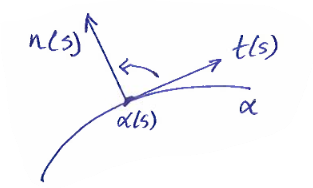
\includegraphics[height=0.5\textheight, width=0.5\textwidth, keepaspectratio]{./Images/flat_curve_03.png}
	\end{center}
\end{figure}
Em particular, como \(t'(s)\) é ortogonal a \(t(s)\), ele também é paralelo a \(n(s)\); logo, vale a relação
\[
	t'(s)=\kappa (s)n(s),
\]
onde \(\kappa (s)\) é a curvatura com sinal da curva \(\alpha \), pois
\[
	\Vert t'(s) \Vert = | \kappa (s) |.
\]
\begin{tcolorbox}[
		skin=enhanced,
		title=Observação,
		fonttitle=\bfseries,
		colframe=black,
		colbacktitle=cyan!75!white,
		colback=cyan!15,
		colbacklower=black,
		coltitle=black,
		drop fuzzy shadow,
		%drop large lifted shadow
	]
	A curvatura mede \textit{o quanto a curva se afasta da sua reta tangente}: se \(\alpha (s) = (x(s), y(s))\) é parametrizada pelo comprimento de arco (doravante p.c.a.), temos
	\begin{align*}
		 & t(s)=(x'(s), y'(s)),    \\
		 & n(s)=(-y'(s), x'(s)),   \\
		 & t'(s)=(x''(s), y''(s)).
	\end{align*}
	Daí, vale a relação
	\[
		\langle t'(s), n(s) \rangle = \langle \kappa (s)n(s), n(s) \rangle = \kappa (s),
	\]
	e, portanto,
	\[
		\kappa (s)=x'(s)y''(s)-x''(s)y'(s).
	\]
\end{tcolorbox}
\begin{exr}
	Prove que \(n'(s)=-\kappa (s)t(s).\)

	%% Como \(\langle n, n \rangle = 1\), vale que \(\langle n', n \rangle = 0\); consequentemente, n' é ortogonal a n, então ele deve paralelo a t, ou seja, \(n'=\lambda t\). 
	% Agora, usando o fato de que \(\langle n, t \rangle = 0\), segue que \(\langle n', t \rangle + \langle n, t' \rangle=0\), ou seja, 
	% \[
	%   \langle \lambda t, t \rangle + \langle n, \kappa n \rangle = 0 \Longleftrightarrow \alpha +k = 0 \Longleftrightarrow \lambda =\kappa . \qedsymbol
	% \]
\end{exr}
\begin{tcolorbox}[
		skin=enhanced,
		title=Lembrete!,
		after title={\hfill Derivando o produto interno},
		fonttitle=\bfseries,
		sharp corners=downhill,
		colframe=black,
		colbacktitle=yellow!75!white,
		colback=yellow!30,
		colbacklower=black,
		coltitle=black,
		%drop fuzzy shadow,
		drop large lifted shadow
	]
	Utilizando a regra de Leibniz, se \(f(x)=(f_1(x),\dotsc , f_{n}(x))\) e \(g(x)=(g_1(x),\dotsc , g_{n}(x))\), do modo que
	\[
		\langle f(x), g(x) \rangle = f_1(x)g_1(x)+\dotsc + f_{n}(x)g_{n}(x),
	\]
	aplicações repetidas dela resultam na relação
	\[
		\langle f, g \rangle = \langle f', g \rangle + \langle f, g' \rangle.
	\]
\end{tcolorbox}
\begin{example}[Reta]
	Seja \(\alpha (s) = p_{0}+sv\), onde s é um número real e v é um vetor unitário, de forma que \(\alpha \) é parametrizada p.c.a. Temos, então,
	\[
		t(s) = v \Rightarrow t'(s) =0, \quad \forall s\in \mathbb{R} \Rightarrow \kappa (s) = 0, \; \forall s\in \mathbb{R}.
	\]
\end{example}
\begin{example}[Círculo]
	Vamos tentar parametrizar e computar a circunferência de um círculo de raio r centrado em \((x_{0}, y_{0})\): para s real e r positivo, considere
	\[
		\alpha (s) = \biggl(r \cos^{}{\biggl(\frac{s}{r}\biggr)}+x_{0}, r\sin^{}{\biggl(\frac{s}{r}\biggr)}+y_{0}\biggr),
	\]
	de modo que
	\[
		t(s)=\alpha '(s) = \biggl(\sin^{}{\biggl(\frac{s}{r}\biggr)}, \cos^{}{\biggl(\frac{s}{r}\biggr)}\biggr)
	\]
	é unitário, ou seja, \(\alpha \) é parametrizada p.c.a. Neste caso, como
	\[
		t'(s)=\biggl(-\frac{1}{r} \cos^{}{\biggl(\frac{s}{r}\biggr)}, -\frac{1}{r}\sin^{}{\biggl(\frac{s}{r}\biggr)}\biggr) = \frac{1}{r}n(s),
	\]
	obtemos a curvatura como
	\[
		\kappa (s) = \frac{1}{r},
	\]
	conforme havíamos conjecturado no início da disciplina.
\end{example}

Nosso próximo passo de estudo é expressar a curvatura para um parâmetro qualquer.  Vamos denotar por s o parâmetro de uma parametrização p.c.a., e por u um parâmetro qualquer de uma curva suave e regular \(\alpha :I\rightarrow \mathbb{R}^{2}\).

Com estas configurações, temos uma parametrização p.c.a, dada por \(\beta (s)=\alpha (\ell^{-1}(s))\) e \(u = \ell^{-1}(s),\) onde
\[
	\ell (u) = \int_{u_{0}}^{u}\Vert \alpha'(t) \Vert \mathrm{d}t.
\]
Consequentemente,
\begin{align*}
	\frac{\mathrm{d}u}{\mathrm{d}s} = \frac{\mathrm{d}}{\mathrm{d}s}(\ell^{-1}(s)) & = \frac{1}{\ell'(\ell ^{-1}(s))}              \\
	                                                                               & = \frac{1}{\Vert \alpha'(\ell^{-1}(s)) \Vert} \\
	                                                                               & = \frac{1}{\Vert \alpha'(u) \Vert},
\end{align*}
mas por termos a regra da cadeia, se considerarmos outra função suave f, obtemos a expressão
\[
	\frac{\mathrm{d}}{\mathrm{d}s}= \frac{\mathrm{d}f}{\mathrm{d}u}\frac{\mathrm{d}u}{\mathrm{d}s}=\frac{1}{\Vert \alpha '(u) \Vert}\frac{\mathrm{d}f}{\mathrm{d}u}
\]
ou seja, podemos traduzir de uma parametrização por s para uma parametrização por u com a relação
\[
	\boxed{\frac{\mathrm{d}}{\mathrm{d}s} = \frac{1}{\Vert \alpha '(u) \Vert}\frac{\mathrm{d}}{\mathrm{d}u}}.
\]
Mais geralmente, escrevendo \(\alpha (u)=(x(u), y(u))\) para a curva \(\alpha \), a expressão de \(t(u)\) torna-se
\[
	t(u) = \frac{\alpha'(u)}{\Vert \alpha'(u) \Vert}=\frac{1}{\sqrt[]{x'(u)^{2}+y'(u)^{2}}}(x'(u), y'(u));
\]
deste modo, omitindo o parâmetro u\footnote{Ou seja, todas as derivadas de x e y serão com respeito ao parâmetro u pelo resto do raciocínio.}, chegamos na relação
\begin{align*}
	\frac{\mathrm{d}t}{\mathrm{d}s} & = \frac{1}{\sqrt[]{x'^{2}+y'^{2}}}\frac{\mathrm{d}}{\mathrm{d}u}\biggl(\frac{1}{\sqrt[]{x'^{2}+y'^{2}}}(x', y')\biggr)                      \\
	                                & = \frac{1}{\sqrt[]{x'^{2}+y'^{2}}}\biggl[\frac{1}{\sqrt[]{x'^{2}+y'^{2}}}(x'', y'') + \biggl(\sqrt[]{x'^{2}+y'^{2}}\biggr)'(x', y')\biggr],
\end{align*}
e, utilizando a expressão
\[
	\kappa (u) = \biggl\langle \frac{\mathrm{d}t}{\mathrm{d}s}, n \biggr\rangle, \quad n = \frac{1}{\sqrt[]{x'^{2}+y'^{2}}}(-y', x'),
\]
chegamos em
\[
	\kappa (u) = \frac{1}{(x'^{2}+y'^{2})^{\frac{3}{2}}}(x'y''-x''y').
\]
Portanto, obtemos uma expressão para a curvatura em termos da parametrização por u:
\[
	\kappa (u) = \frac{(x'y''-x''y')}{(x'^{2}+y'^{2})^{\frac{3}{2}}}.
\]
\subsection{Pontos de Inflexão e Vértices}
\begin{def*}
	Um ponto \(u_{0}\) de uma curva \(\alpha :I\rightarrow \mathbb{R}^{2}\) é chamado \textbf{ponto de inflexão} se \(\kappa (u_{0})=0\); se, por outro lado, \(\kappa'(u_{0})=0\), então chamaremos o ponto \(u_{0}\) de \textbf{vértice}. \(\square\)
\end{def*}
\begin{example}
	Vamos tomar a curva \(\alpha (u)=(u, u^{3}),\; u\in \mathbb{R}\), cujo traço é
	\begin{figure}[H]
		\begin{center}
			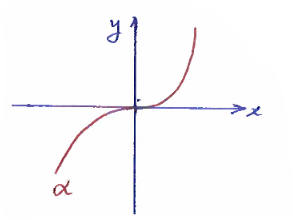
\includegraphics[height=0.5\textheight, width=0.5\textwidth, keepaspectratio]{./Images/inflection_04.png}
		\end{center}
	\end{figure}
	Aqui, temos as relações parametrizadas
	\[
		\left.\begin{array}{ll}
			\alpha '(u)=(1, 3u^{2}) \\
			\alpha ''(u)=(0,6u)
		\end{array}\right\} \Rightarrow \kappa (u)=\frac{6u}{(1+9u^{4})^{\frac{3}{2}}}.
	\]
	Quais são os pontos de inflexão dessa curva? Ela tem algum vértice?

	Para começar, observe que o denominador nunca se anula (naturalmente), mas o numerador sim, quando \(u=0\); logo,
	\[
		\kappa (u)=0 \Longleftrightarrow u =0,
	\]
	donde concluímos que \(\alpha (0)=(0,0)\) é um ponto de inflexão de \(\alpha \).
	Ademais,
	\[
		\kappa '(u) = -\frac{270x^{4}-6}{(9x^{4}+1)^{\frac{5}{2}}},
	\]
	que se anula quando \(270x^{4}-6=0.\)
\end{example}
\end{document}

